Hvis man vil komprimere en datamængde ved brug af Huffman coding, kræver det, at der bliver lavet et huffman træ. Dette træ kan genereres på tre forskellige måder: Statisk, dynamisk eller adaptivt. Principielt ser det resulterende bit-træ ens ud for hver af metoderne. Det handler mere om hvordan træerne bliver genereret. I dette afsnit vil der være en gennemgang, af hvordan disse metoder virker, samt deres fordele og ulemper i forhold til SMS-beskeder. Den følgende tabel samt den følgende figur viser, hvordan et potentielt Huffman bit-træ kunne se ud.

\begin{table}[H]
\begin{center}
\begin{tabular}{|c|c|}
\hline
\cellcolor{ForestGreen}\color{white}{\textbf{Tegn}}& \cellcolor{ForestGreen}\color{white}{\textbf{Forekomster}}\\[2ex] \hline
A & 24 \\ \hline
B & 12 \\ \hline
C & 10 \\ \hline
D & 8 \\ \hline
E & 8 \\ \hline
\end{tabular} 
\caption{Et sæt tegn og forekomster}
\end{center}
\end{table}

\begin{figure}[H]
\centering
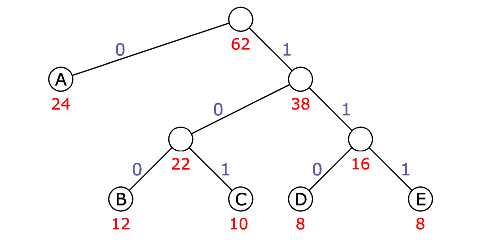
\includegraphics[width=0.75\linewidth]{Billeder/huffman_tree.png}
\caption{Det samme sæt som før set i et Huffman træ \cite{Hufftree_1}}
\label{fig:huffmantree_fred}
\end{figure}

Ud fra billedet kan man se, at de tegn som forekommer færrest gange, er placeret nederst i træet, D og E, mens det tegn som forekommer mest er placeret øverst, A. Hver gang man går et niveau ned så går længden på et tegn op. A har en længde på 1 bit mens B, C, D og E har en længde på 3 bit. Tegnet som forekommer mest, får altså den mindste længde. Derudover kan man også ud fra figur \ref{fig:huffmantree_fred} se det følgende binære talsystem:

\begin{table}[H]
\begin{center}
\begin{tabular}{|c|c|c|}
\hline
\cellcolor{ForestGreen}\color{white}{\textbf{Tegn}} & \cellcolor{ForestGreen}\color{white}{\textbf{Binær Kode}} & \cellcolor{ForestGreen}\color{white}{\textbf{Kode Længde}}\\[2ex] \hline
A & 0 & 1 \\ \hline
B & 100 & 3 \\ \hline
C & 101 & 3 \\ \hline
D & 110 & 3 \\ \hline
E & 111 & 3 \\ \hline
\end{tabular} 
\caption{Binært talsystem fra et Huffman træ}
\end{center}
\end{table}

Dette sæt af tegn og forekomster fylder i alt 496 bit for sig selv, før det er blevet komprimeret, hvis man går ud fra hvert tegn fylder 1 byte, altså 8 bit. I et Huffman træ som dette billede viser, fylder de samme tegn 138 bit, som kan findes ved at lægge tegnene sammen i forhold til deres forekomster og længder plus selve træet hvis det er et dynamiske træ. På figur \ref{fig:huffmantree_fred} kan man også se punkter, som ikke indeholder nogen tegn. Disse punkter kaldes for knuder, og har en størrelse magen til summen af punkterne nedenunder den. Den øverste knude hvor træet altid starter kaldes for roden. Enderne på træet som indeholder de egentlige tegn kaldes for blade.

\subsection{Statisk}
Den første metode man kan bruge til at generere et Huffman træ, er den statiske metode. Et statisk Huffman træ bliver lavet ud fra formodede forekomster på i et stykke tekst. For eksempel hvis man kigger generelt på det engelske sprog, så forekommer tegnet ’e’ mest, og vil derfor blive placeret øverst i det statiske Huffman træ, mens tegn som ’z’ og ’x’ vil blive placeret nederst. Den statisk opbygning af et Huffman træ er standard metoden\cite{Hufftree_2}.

Et statisk Huffman træ virker på alle stykker tekst, især længere stykker af tekst som for eksempel artikler. Til gengæld kan den ende med at ikke gøre fuld brug af komprimeringskraften ved Huffman coding, når det handler om mindre beskeder, fordi det ikke altid går op med normalen for tegn forekomster i et sprog. Statiske Huffman træer virker bedre, i takt med at den tekst som skal komprimeres bliver større, og bliver mere ineffektiv, når teksten bliver mindre. Det er ikke sandsynligt, at den komprimerede tekst vil fylde mere, end hvis den ikke var komprimeret idet at Huffman komprimering er så effektivt som det er. \cite{Hufftree_3}

Fordele ved et statisk træ er at det let kan give gode resultater for større stykker af tekst og behøver ikke at sende noget yderligt i beskeden udover bitmønstret. Et statisk træ er også hurtigt idet at der ikke er behov for at generer et nyt træ for hvert eneste stykke tekst, som der er behov for med de to kommende metoder. Statisk kan derfor have en fordel fordi den ikke behøver ligeså meget regnekraft på enheder som mobiltelefoner, som muligvis kan være begrænset på det område.


\subsection{Dynamisk}
Den anden metode man kan bruge kaldes for et dynamisk Huffman træ. Et dynamisk træ bliver generet ud fra det reelle data som teksten består af. Træet bliver genereret ud fra den specifikke besked og er ikke en generel liste som ved den statiske metode. Det dynamiske træ er derfor den mest optimale til Huffman coding. Den dynamiske opbygning af et træ starter med at sætte de to tegn med færrest forekomster til en knude. Derefter bliver der bygget ovenpå den knude og tager hele tiden de tegn med færrest forekomster som endnu ikke er blevet sat ind i træet. En ny knude bliver lavet som får sat det næste tegn samt den foregående knude som indeholder alle tidligere tegn og knuder på.

\begin{figure}[H]
\centering
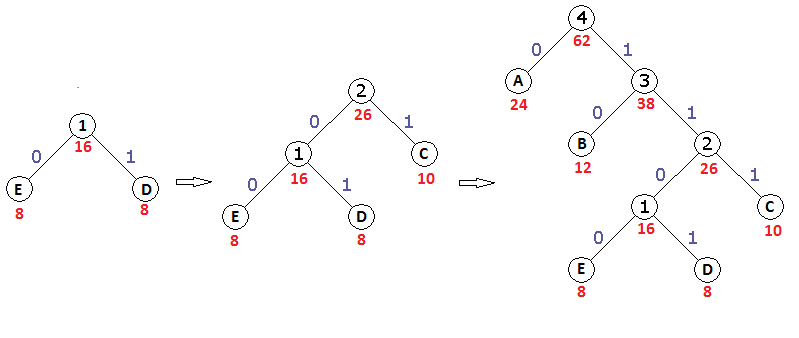
\includegraphics[width=\linewidth]{Billeder/dynamisk.png}
\caption{Dynamisk opbygning af et Huffman træ udfra det tidligere eksempel}
\label{fig:dynamic_tree}
\end{figure}

En ulempe ved den dynamiske metode er, at for at kunne dekode den komprimeret tekst  skal man bruge en kode tabel over træet. Idet at det er et træ skræddersyet til et bestemt stykke tekst, så har dem der skal dekode teksten ingen mulighed til hvordan man oversætter 0 og 1 tallene tilbage til den oprindelige tekst. Derfor er det nødvendigt med den dynamiske metode at medsende en tabel som angiver hvilke tegn har hvilke bitmønstre. Dette betyder selvfølgelig at den komprimeret tekst fylder et stykke mere og gør derfor ikke optimalt brug af komprimerings kraften ved Huffman coding. \cite{Hufftree_4}

Fordelen ved et dynamisk træ i forhold til det statiske er at den mere konstant gør optimal brug af Huffman coding til at komprimere et stykke tekst. Det er selvfølgelig det man gerne vil opnå i forhold til SMS beskeder, men som sagt så er det nødvendigt at sende en tabel med så det er muligt at dekode det komprimeret stykke tekst. Dette betyder at SMS beskeden fylder mere end hvis det bare var det komprimeret stykke tekst, og arbejder derfor imod målet om at formindske størrelsen af den data der bliver sendt.

\subsection{Adaptivt}
Den tredje og sidste metode til at komprimere et stykke tekst med Huffman coding er den adaptive metode. Med den adaptive metode starter træet med at intialisere forekomsten af tegn som de kommer til 1. Når det samme tegn fremkommer igen så vil det blive lagt til tegnets fremkomst værdi, og træet vil derefter også opdatere sig selv sådan hvis et nyt tegn begynder at have flest forekomster så vil den blive placeret øverst i træet.
I forhold til den foregående metode så kan den adaptive metode genere et træ alt efter hvad for noget data som skal komprimeres, ligesom den dynamiske metode, men har til gengæld ikke behov for at videregive en tabel som viser hvordan man oversætter det komprimerede tekst, idet at det adaptive træ på den enhed som dekomprimere vil gøre arbejdet og opdatere sig selv med det data den dekomprimere. Dette kan også betyde at det dynamiske træ muligvis ikke behøver at sende en tabel med over hvis dekomprimeringen sker ved hjælp af det adaptive træ. Ulempen ved den adaptive metode er at det stykke tekst der bliver komprimeret eller dekomprimeret ikke indgår i den nuværende version af træet, idet at det adaptive træ først opdateres med data fra tekststykket efter det er blevet komprimeret eller dekomprimeret. Derudover så kræver den også meget regnekraft fra den enhed som skal komprimere og dekomprimere fordi den konstant skal opdateres af det data den gennemarbejder. \cite{Hufftree_5}
I forhold til SMS beskeder så er den adaptive metoder sikkert bedst når det kommer til at formindske den mængde data der bliver sendt med beskeden. Ulempen er dog at træet har brug for tid til at komme op og køre ved at konstant opdatering af sit eget træ. Den adaptive metode starter derfor ud med at være langsom og ineffektivt idet at den introducere alle tegn fra bunden af og kan først effektivt komprimere efter den har arbejdet sig igennem et antal tekststykker. Kravet for regnekraft på enhederne der komprimere og dekomprimere  kan også være en større ulempe på en mobiltelefon.

\subsection{Sammenligning}
Alle tre modeller har sine fordele og ulemper. I dette afsnit der blive delkonkluderet på hele af afsnittet, og hver model vil blive sammenlignet med hinanden, og til resten af projektet, for at finde den model som bedst kan bruges til at besvare problemformuleringen omkring SMS beskeder.

Først er der den statiske model. Som sagt, så kræver den statiske model ikke særlig meget regnekraft. Derudover så er den også let at implementere fordi det er, som navnet hentyder, et statisk træ og er derfor altid ens. Ulempen ved den statiske model er at den ikke altid kan gøre optimalt brug af Huffman coding. Den tekst der skal komprimeres stemmer ikke altid overens med forekomst ratioen og kan derfor ikke gøre perfekt brug af Huffman. På dette punkt er både den dynamiske og den adaptive model bedre som kan lave sine egne træer alt efter hvad der skal komprimeres.

Med det kommer den dynamiske model. Af de tre modeller gør den dynamiske model bedst brug af komprimeringskraften ved Huffman coding idet at den laver et helt nyt træ ud fra det tekststykke den skal komprimere. Den dynamiske model har dog en del implementerings ulemper. Som sagt, så skal der sendes en manual med, som optager plads, for at kunne dekomprimere tekststykket igen. Derudover så kræver den dynamiske model også en del ekstra regnekraft på enheden for at generer et nyt træ hver gang der skal sendes en besked.

Den sidste model er den adaptive model. Fordelen ved den adaptive model er at den gør god brug af Huffman coding som den dynamiske model, og behøver ikke at sende noget ekstra med for at sikre modtageren kan dekomprimere beskeden, som den statiske model.Ulempen ved den adaptive model er at den ikke altid kan gøre optimalt brug af Huffman coding idet at træet først opdateres efter den har komprimeret og dekomprimeret et tekststykke. Derudover så er det også den model som kræver mest arbejde for at virke, og tager mest regnekraft på enheden.

Til sidst kommer spørgsmålet så igen; Hvilken model vil være bedst til at bruge i besvarelsen af projektets problemformulering? For det første så kræver både den dynamiske og den adaptive model langt mere regnekraft, i forhold til den statiske, for at kunne fungere. Dette kan give problemer idet programmet skal kunne køre på mobiltelefoner. Det er også blevet vist at komprimering med Huffman er meget effektivt, så tabet i komprimering ved at bruge den statiske og den adaptive model er ikke alt for væsentlig. Derudover så bliver komprimeringen mere effektiv, alt efter hvor lang tekststykket er, og målet med projektet var at kunne komprimere SMS beskeder som overstiger tegnbegrænsningen. Den statiske og den adaptive model behøver heller ikke at bruge ekstra plads, som den dynamiske gør, for at sikre at beskeden kan blive dekomprimeret igen. Ud fra disse punkter, samt sammenligningen og resten af afsnittet, blev det bestemt at løsningen skulle laves ved hjælp af et statisk Huffman træ.
